\documentclass{beamer}
\usepackage{etex}
\usepackage[utf8]{inputenc}
\usepackage[T1]{fontenc}
\usepackage[english]{babel}
\usepackage{amssymb}
\usepackage{verbatim}
\usepackage{beamerthemesplit}
\usepackage{graphicx}
\usepackage{listings}
\usepackage{figlatex}

\beamertemplatetransparentcovereddynamic

\lstdefinestyle{CStyle}{
        language=C,
        backgroundcolor=\color{white},
        commentstyle=\color{gray},
        keywordstyle=\color{magenta},
        numberstyle=\tiny\color{gray},
        stringstyle=\color{purple},
        basicstyle=\tiny,
        morekeywords={cl_uint,cl_platform_id,cl_device_id,cl_context_properties,cl_context,cl_program,cl_kernel,cl_command_queue,cl_mem,size_t},
        breakatwhitespace=false,
        breaklines=true,
        captionpos=b,
        keepspaces=true,
        numbers=left,
        numbersep=5pt,
        showspaces=false,
        showstringspaces=false,
        showtabs=false,
        tabsize=2
}

\lstdefinestyle{CPPStyle}{
        language=C++,
        backgroundcolor=\color{white},
        commentstyle=\color{gray},
        keywordstyle=\color{magenta},
        numberstyle=\tiny\color{gray},
        stringstyle=\color{purple},
        basicstyle=\tiny,
        breakatwhitespace=false,
        breaklines=true,
        captionpos=b,
        keepspaces=true,
        numbers=left,
        numbersep=5pt,
        showspaces=false,
        showstringspaces=false,
        showtabs=false,
        tabsize=2
}

\lstdefinestyle{OpenCLStyle}{
        language=C,
        backgroundcolor=\color{white},
        commentstyle=\color{gray},
        keywordstyle=\color{magenta},
        numberstyle=\tiny\color{gray},
        stringstyle=\color{purple},
        basicstyle=\tiny,
        morekeywords={__private,__local,__global,__constant,__kernel,__read_only,__write_only,__read_write},
        breakatwhitespace=false,
        breaklines=true,
        captionpos=b,
        keepspaces=true,
        numbers=left,
        numbersep=5pt,
        showspaces=false,
        showstringspaces=false,
        showtabs=false,
        tabsize=2
}

\usecolortheme{progressbar}
\usefonttheme{progressbar}
\useoutertheme{progressbar}
\useinnertheme{progressbar}

\graphicspath{{figures/}}

\title{Layers for OpenCL}
\author{Brice Videau (Argonne National Laboratory)}

\begin{document}

\frame{\titlepage}

\section{Introduction and Problematic}

\subsection{Introduction}

\frame{
  \frametitle{Application Complexity}
  \begin{columns}
    \column{5.5cm}
    \begin{block}{More Complex Environment}
      \begin{itemize}
      \item Hardware is becoming increasingly heterogeneous,
      \item Application have adapted by adding additional layers of abstraction
            between programmers and the hardware they target,
      \item Sometimes difficult to understand and debug these applications.
      \end{itemize}
    \end{block}
    \column{5.5cm}
    \begin{block}{Libraries are a Window into Applications}
      \begin{itemize}
      \item Applications rely on libraries as bridge to the hardware,
      \item Libraries present consistent \textit{Application Programming
            Interfaces} APIs,
      \item Library APIs define \textit{programming models},
      \item Programming Model usage can be \textit{validated}
      \end{itemize}
    \end{block}
  \end{columns}
}

\frame{
  \frametitle{Programming Model's Usage Validation}
  
  \begin{block}{What information is required to validate a programming model's
                usage? (sorted by increasing cost/complexity)}
    \begin{itemize}
    \item What functions of the API are called and when,
    \item With what parameters they were called, and what was returned,
    \item To what data were those parameters referring to,
    \item What was the previous state of the programming model.
    \end{itemize}
  \end{block}
  \begin{block}{Example: validate \textit{malloc/free} usage}
  \begin{itemize}
  \item trace memory allocations and store returned pointers in a set,
  \item trace memory release, check that pointer is in the set and remove it.
  \end{itemize}
  \end{block}
  \textbf{Can these goals be achieved outside the application?}\\
  \textbf{Can we modify, the behavior of the programming model?}
}

\subsection[Instrumentation]{Instrumentation: Layers vs Interception}

\frame{
  \frametitle{Library Interception}
  For shared library, \textit{interception} (or interposition) is usually used.
  \begin{itemize}
    \item Create a shared library that implements functions to be traced or
modified
    \item use the real library underneath (several strategies exist here),
    \item Use the dynamic linker to \textit{preload} this library.
  \end{itemize}
  \begin{center}
  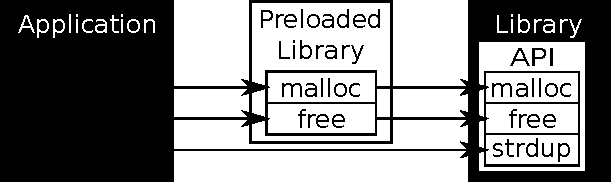
\includegraphics{interception}
  \end{center}
  Famous Example: \textbf{Intel}'s
  \href{https://github.com/intel/opencl-intercept-layer}{\color{blue}
  \underline{Intercept Layer for OpenCL Applications}}
}

\frame{
  \frametitle{Library Interception: Limitations}
  Several limitations come with interception:
  \begin{itemize}
  \item Intercepting calls depends on platform specific functionalities,
  \item Chaining interception libraries can prove difficult if they don't follow
        the same protocol,
  \item Depending on the methods used, there can be quite a lot of boiler-plate
        code involved.
  \end {itemize}
  \textbf{Can we alleviate some of these issues?}
}

\frame{
  \frametitle{Layers as Plugins}
  \textbf{What if this interception could be provided as a plugin by the library
          itself?}

  Examples: Layers for the Vulkan API, PMPI, OMPT, ...
  \begin{block}{Benefits}
    \begin{itemize}
      \item Factoring of platform specific concerns,
      \item Factoring of boilerplate code,
      \item Clear protocol to load layers,
      \item Standardized API for layer development.
    \end{itemize}
  \end{block}
  Design and implement \textbf{Layers for OpenCL}.
  
}

\section{Design and Implementation}

\frame{
  \frametitle{Design and Implementation}
  \begin{center}
  How does the OpenCL \textit{Installable Client Driver} (ICD) Loader work?
  \end{center}
}

\subsection[API Call]{Original OpenCL ICD Loader API Call Workflow}

\frame{
  \frametitle{Original OpenCL ICD Loader API Call Workflow}
  The OpenCL ICD loader is a router for OpenCL calls, directing them to the
correct vendor driver:
  \begin{center}
  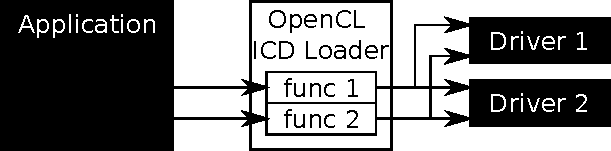
\includegraphics{ICD_Loader}
  \end{center}
}

\begin{frame}[fragile]
  \frametitle{In the Beginning Was the Dispatch Table...}
  In order to support several implementations simultaneously, OpenCL Object are
  required to conform to this definition:
  \lstset{style=CStyle}
  \begin{lstlisting}
/* Dispatch table providing pointers to vendor
 * implementation of the OpenCL API
 */
typedef struct _cl_icd_dispatch {
  /* OpenCL 1.0 */
  cl_api_clGetPlatformIDs clGetPlatformIDs;
  cl_api_clGetPlatformInfo clGetPlatformInfo;
  cl_api_clGetDeviceIDs clGetDeviceIDs;
  cl_api_clGetDeviceInfo clGetDeviceInfo;
  /* ... */
}
struct _cl_device_id { cl_icd_dispatch *dispatch; };
typedef struct _cl_device_id *cl_device_id;
\end{lstlisting}
  Objects carry around references (function pointers) to the functions (API
  entry points) that need to be used with those objects.
\end{frame}

\begin{frame}[fragile]
  \frametitle{Original OpenCL Loader API Dispatch Example}
  The OpenCL ICD Loader's job is to:
  \begin{itemize}
    \item check for \textit{NULL} handle,
    \item call the correct function in the dispatch table.
  \end{itemize}
  \lstset{style=CStyle}
  \begin{lstlisting}
cl_int clGetDeviceInfo(cl_device_id device,
   cl_device_info param_name, size_t param_value_size,
   void* param_value, size_t* param_value_size_ret)
{
  if (!device) return CL_INVALID_DEVICE;
  return device->dispatch->clGetDeviceInfo(device,
    param_name, param_value_size,
    param_value, param_value_size_ret);
}
  \end{lstlisting}
\end{frame}

\subsection[Layer API Call]{OpenCL ICD Loader with Layers API Call Workflow}

\frame{
  \frametitle{OpenCL ICD Loader with Layers API Call Workflow}
  With layer support enabled, the OpenCL ICD loader will first redirect calls to
  the different active layers, then directs the call to the correct vendor
  driver:
  \begin{center}
  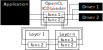
\includegraphics{ICD_Loader_Layers}
  \end{center}
}

\subsection[Implementation]{OpenCL ICD Loader Layers Implementation}

\frame{
  \frametitle{OpenCL ICD Loader Layers Implementation}
}

\section{Layer Usage and Development}
\subsection[configuration]{OpenCL ICD Loader Layers Configuration Options}

\frame{
  \frametitle{OpenCL ICD Loader Layers Configuration Options}
}

\subsection[Layer API]{OpenCL Layers Plugin API}

\frame{
  \frametitle{OpenCL Layers Plugin API}
}

\section[Conclusion]{Conclusion and Perspectives}

\frame{
  \frametitle{Conclusion and Perspectives}
}

\end{document}
